\subsection{Datenauswertung} \label{cap:methoden_datenauswertung}

Anhand eines lauten Geräusches (z.B. Schlag auf den Tisch) können die Aufnahmen von den Kapiteln \ref{cap:methoden_drehzahlmessung} \&  \ref{cap:methoden_magnetbremsung}) in einem Filmbearbeitungsprogramm synchronisiert werden und die Daten herausgelesen werden. Dies ist natürlich kein professioneller Weg, diese Zeit zu überprüfen, aber sie funktionierte einwandfrei, mit den Geräten, welche zur Verfügung standen.
\newpara
Der Vorteil daran ist, dass anhand der Bildrate des Films die Zeiten zwischen zwei Bildern konstant und berechenbar sind. Jede Messungsaufnahme besitzt eine Bildrate von 30 Bildern pro Sekunde. Wird nun eine Sekunde durch 30 geteilt, erhält man die Zeit $0.0\overline{3}s$ (Siehe Formel \ref{equ:time_datenauswertung}).

\begin{equation}
    \label{equ:time_datenauswertung}
    t=\frac{t}{Anzahl Bildern}=\frac{1s}{30}=0.0\overline{3}s \tag{25}
  \end{equation}
  \begin{gather}
  \shortintertext{\textbf{Begriffe:}}
  \begin{tabularx}{0.9\textwidth}{ll}
$n_1$    &   Anfangsdrehzahl\\
$n_2$    &   Enddrehzahl\\
  \end{tabularx}\nonumber
\end{gather}

Als Filmbearbeitungsprogramm wurde Davinci Resolve von Blackmagic-Design verwendet. Wichtig war es, ein Programm zu verwenden, welches ein Projekt als einzelne Bilder exportieren kann. Ein Projekt wird erstellt und die Kamera- und Laptopaufnahme wird in die Medien-Bibliothek aufgenommen. Diese werden nun in die Timeline hineingezogen und aufeinandergelegt. Eine Aufnahme wird solange verschoben, bis alle Geräusche synchron klingen (kein Echo).



\begin{figure}[ht]
    \begin{center}
      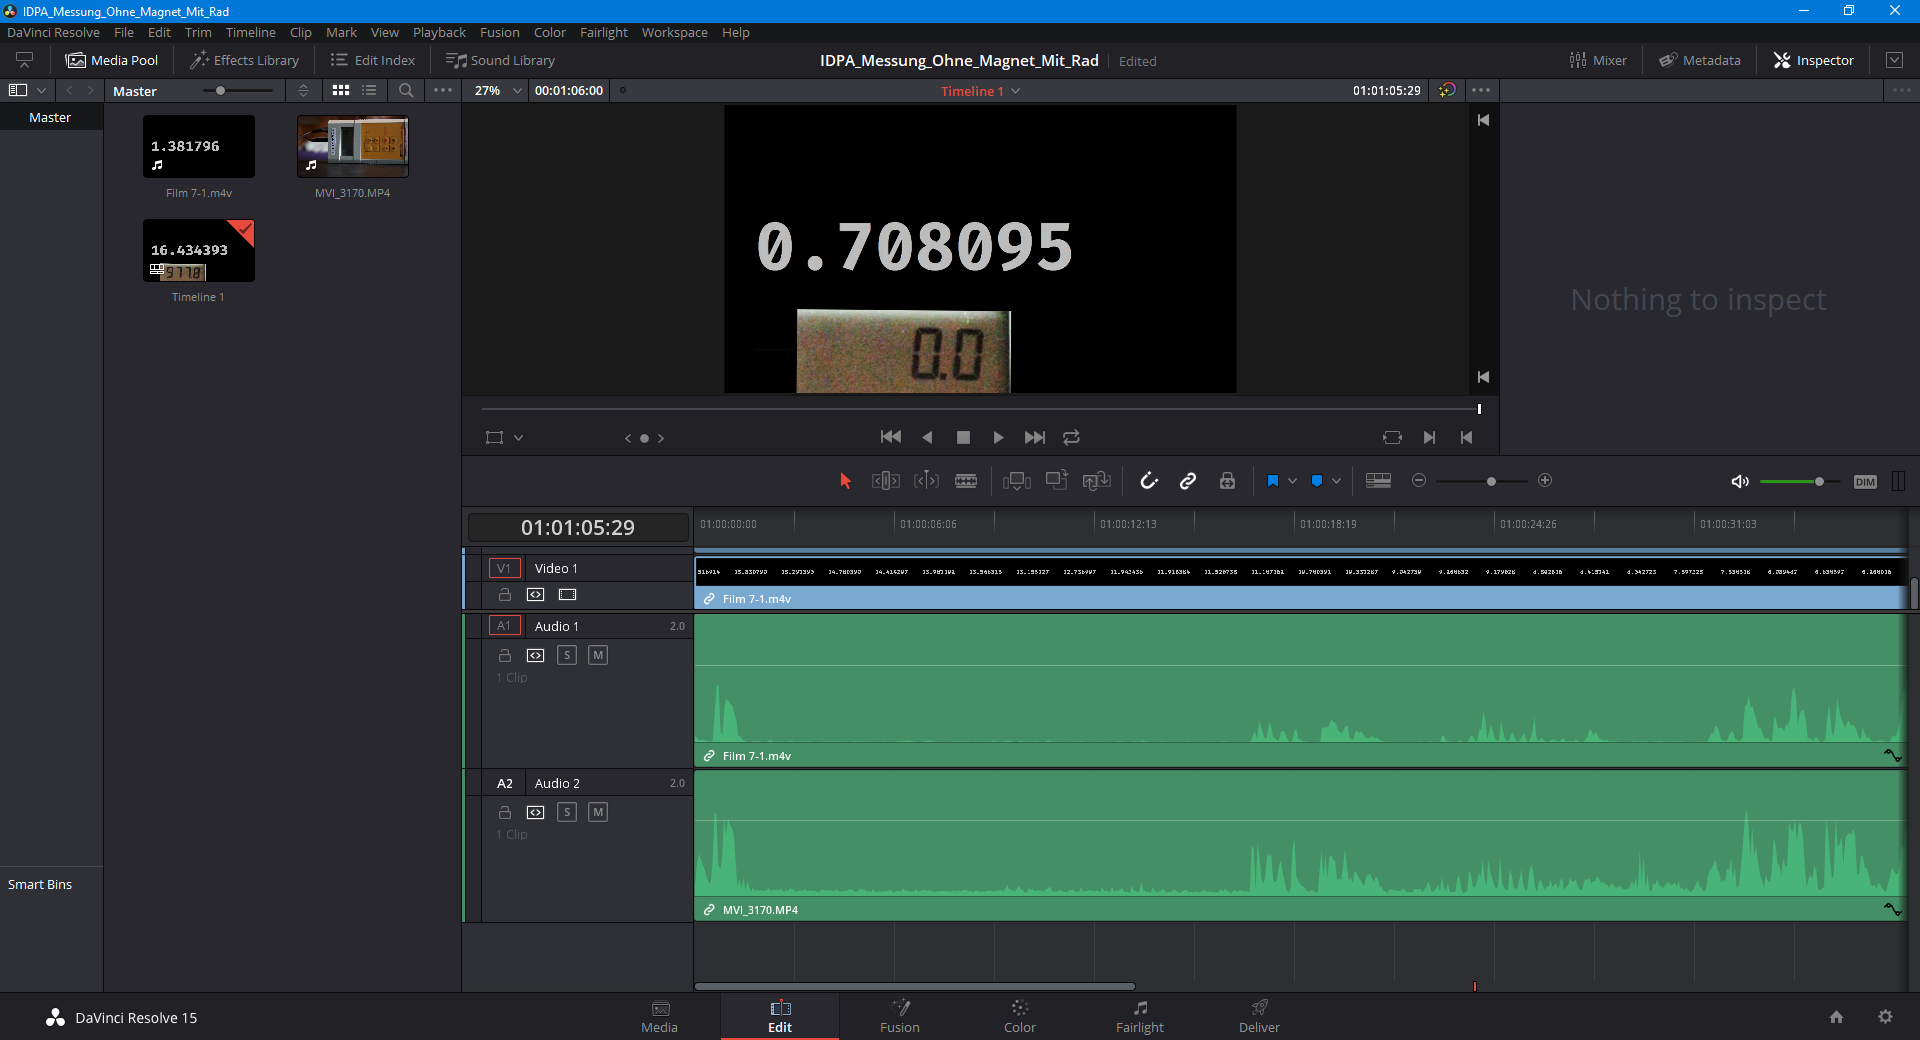
\includegraphics[width=14cm]{assets/images/resolve_mediapool}
    \end{center}
    \vspace{-3ex}
    \caption{Ausschnitt aus Davinci Resolve}
    \label{fig:resolve_mediapool}
  \end{figure}

Als Filmbearbeitungsprogramm wurde \textit{Davinci Resolve} von \textit{Blackmagic-Design} verwendet. Wichtig war es, ein Programm zu verwenden, welches ein Projekt als einzelne Bilder exportieren kann. Ein Projekt wird erstellt und die Kamera- und Laptopaufnahme wird in die Medien-Bibliothek aufgenommen. Diese werden nun in die \textit{Timeline} hineingezogen und aufeinandergelegt. Eine Aufnahme wird solange verschoben, bis alle Geräusche synchron klingen (kein Echo) (siehe Abbildung \ref{fig:resolve_mediapool}).
\newpara
Wurde dieser Schritt gemacht, wird das Video als TIFF bei der kleinsten Auflösung (720 x 480 Pixel) exportiert. Als Endprodukt erhält man einzelne Bilder, die je nach Länge des Videos variieren (siehe Formel \ref{equ:anzahl_bilder_resolve}).

\begin{equation}
    \label{equ:anzahl_bilder_resolve}
    Anzahl Bilder=t_{Video}\cdot f_{fps} \tag{26}
  \end{equation}
  \begin{gather}
  \shortintertext{\textbf{Begriffe:}}
  \begin{tabularx}{0.9\textwidth}{ll}
$t_{Video}$    &   Länge des Videos\\
$f_{fps}$    &   Bildrate des Videos\\
  \end{tabularx}\nonumber
\end{gather}
Das längste Video beträgt eine Länge von ca. 3 Minuten, was ca. 5400 Bildern entspricht. Zur Auswertung sind dies zu viele Bildern, da die Werte von Hand in eine Excel Tabelle eingetragen werden müssen. Für dieses Projekt wird es keine gravoeremdem Folgen haben, wenn die Anzahl Bilder gekürzt wird. Es wird daher eine maximale Menge von 250 Bildern pro Messung gesetzt. Bei 250 Bildern können grosse Änderungen immer noch erkannt werden, dafür aber keine Feinänderungen.
\newpara
Werden die exportierten Bilder auf 250 Stück gekürzt, wird sich auch die Zeit zwischen zwei Bildern ändern (Siehe Formel \ref{equ:faktor_bilder} \& \ref{equ:zeit_verlangsamung}). Wird als Beispiel ein Faktor von 32 berechnet und das Video besitzt eine Bildrate von 30 Bildern pro Sekunde, würde eine Zeit von 1.0¯6s berechnet.

\begin{equation}
    \label{equ:faktor_bilder}
    x=\frac{x_{BilderTotal}}{x_{BilderSoll}} \tag{27} 
  \end{equation}
  \begin{equation}
    \label{equ:zeit_verlangsamung}
    t_{fps}=\frac{x}{f_{fps}} \tag{28} 
  \end{equation}
  \begin{gather}
  \shortintertext{\textbf{Begriffe:}}
  \begin{tabularx}{0.9\textwidth}{ll}
    $x$	        &   Bilder-Verkleinerungs-Faktor\\
    $x_{Total}$ &	Totale Anzahl Bilder des exportierten Videos\\
    $x_{Soll}$  &	Gewünschte Anzahl Bilder\\
    $t_{fps}$   &	Zeit zwischen zwei Bildern\\
    $f_{fps}$   &	Bildrate\\
  \end{tabularx}\nonumber
\end{gather}

Sind alle Bilderserien vorbereitet, können die Daten auf den Bildern in ein Excel eingetragen werden und verarbeitet werden.